\documentclass[a4paper,10pt]{article}

% Pacchetti per la matematica e simboli
\usepackage{amsmath}    % Formule matematiche
\usepackage{amssymb}    % Simboli matematici
\usepackage{amsfonts}   % Font matematici
\usepackage{mathrsfs}   % Scrittura calligrafica matematica
\usepackage{amsthm}     % Teoremi e definizioni
\usepackage{algorithm}
\usepackage{algpseudocode}
\usepackage{listings} % Per il codice
\usepackage{xcolor} % Per colorare il codice

% Configurazione del pacchetto listings


% Pacchetti per grafici
\usepackage{graphicx}   % Inclusione grafica
\usepackage{tikz}       % Disegni e grafici
\usepackage{pgfplots}   % Grafici avanzati
\pgfplotsset{compat=1.18} % Imposta compatibilità per pgfplots

% Pacchetti per la gestione degli indici e riferimenti
\usepackage{hyperref}   % Riferimenti ipertestuali
\hypersetup{
    colorlinks=true,    % Colori per i link
    linkcolor=darkblue, % Colore dei link interni
    citecolor=darkblue, % Colore dei riferimenti alle citazioni
    filecolor=darkblue, % Colore dei link ai file
    urlcolor=darkblue,  % Colore degli URL
    pdftitle={Formulario di Analisi Reale},
    pdfpagemode=UseOutlines
}
\usepackage{tocbibind}  % Include l'indice e la bibliografia nel sommario
\usepackage{fancyhdr}   % Intestazioni e piè di pagina personalizzati
\usepackage{bookmark}   % Gestione segnalibri PDF

% Impostazioni dei margini
\usepackage{geometry}
\geometry{
    left=0.5in,
    right=0.5in,
    top=0.5in,
    bottom=1in
}

% Gestione delle sezioni e sottosezioni
\usepackage{titlesec}
\titleformat{\section}[block]{\large\scshape}{\thesection}{1em}{} % Titoli sezioni maiuscoli
\titleformat{\subsection}[block]{\normalsize\bfseries}{\thesubsection}{1em}{}
\titleformat{\subsubsection}[block]{\normalsize\itshape}{\thesubsubsection}{1em}{}
\titleformat{\paragraph}[runin]{\normalsize\bfseries}{\theparagraph}{1em}{}[:]
\titleformat{\subparagraph}[runin]{\normalsize\itshape}{\thesubparagraph}{1em}{}[:]

% Colore e aspetto
\usepackage{xcolor}
\definecolor{darkblue}{rgb}{0.0, 0.2, 0.6}
\definecolor{gray}{rgb}{0.5, 0.5, 0.5}

% Teoremi e definizioni formali
\newtheoremstyle{mystyle} % Definisci lo stile del teorema
  {10pt} % Spaziatura sopra
  {10pt} % Spaziatura sotto
  {\itshape} % Corpo del teorema in corsivo
  {} % Indentazione del numero
  {\bfseries} % Font del titolo
  {}     % Punteggiatura dopo il titolo
  {\newline} % Spazio dopo il titolo
  {}     % Stile del testo

\theoremstyle{mystyle}
\newtheorem{theorem}{Teorema}[section]
\newtheorem{definition}[theorem]{Definizione}
\newtheorem{lemma}[theorem]{Lemma}
\newtheorem{corollary}[theorem]{Corollario}
\newtheorem{proposition}[theorem]{Proposizione}

% Pacchetti aggiuntivi
\usepackage{enumitem}   % Gestione elenchi personalizzati
\usepackage{multicol}   % Colonne multiple
\usepackage{booktabs}   % Tabelle formattate professionalmente
\usepackage{caption}    % Migliore gestione delle didascalie
\captionsetup{
    labelfont=bf,
    font=small,
    labelsep=colon
}

% Impostazioni di line spacing
\usepackage{setspace}
\onehalfspacing  % Interlinea 1.5 per migliorare la leggibilità

% Informazioni del documento
\title{\textbf{Elaborazione dei segnali}}
\author{\textit{Oudeys}}
\date{\today}

% Impostazione del titolo dell'indice
\renewcommand{\contentsname}{Indice}

% Dimensioni delle formule
\DeclareMathSizes{6}{6}{6}{6} % Imposta dimensioni per le formule
\usepackage{setspace}
\singlespacing  % Interlinea singola per ridurre lo spazio tra le righe

% Inizio del documento
\begin{document}

\maketitle

\newpage


\tableofcontents
\newpage

\part{Teoria dei segnali}
\begin{multicols}{2}

\section{Proprietà dei segnali}

\begin{definition}[Segnale causale]
    \[
    x(t) =
    \begin{cases}
        x_s(t) & \forall \ t \geq t_0 \\
        0 & \forall \ t < t_0
    \end{cases}
    \]
\end{definition}

\subsection{Forme d'onda elementari}

\begin{definition}[Funzione rettangolo simmetrico]
\(
A \Pi \left( \frac{t}{T} \right) =
\begin{cases}
    A & \forall \lvert t \rvert < T/2 \\
    0 
\end{cases}
\)
\begin{center}
    \begin{tikzpicture}
        % Asse x
        \draw[->] (-4,0) -- (4,0) node[right] {$t$};
        % Asse y
        \draw[->] (0,-0.5) -- (0,2) node[above] {$A \Pi \left(\frac{t}{T} \right)$};
    
        % Grafico della funzione rettangolo
        \draw[thick, blue] (-2, 1) -- (2, 1);
        \draw[thick, blue] (2, 1) -- (2, 0);
        \draw[thick, blue] (-2, 1) -- (-2, 0);
        \draw[thick, blue] (2, 0) -- (4, 0);
        \draw[thick, blue] (-4, 0) -- (-2, 0);
    
        % Punti di annotazione
        \draw[dashed] (-2, 0) -- (-2, 1);
        \draw[dashed] (2, 0) -- (2, 1);
    
        % Annotazioni
        \node[below] at (-2, 0) {$-\frac{T}{2}$};
        \node[below] at (2, 0) {$\frac{T}{2}$};
        \node[left] at (0, 1.3) {$A$};
    \end{tikzpicture}
\end{center}
\end{definition}




\begin{definition}[Funzione gradino unitario]
\(
u(t) =
\begin{cases}
    1 & \forall t \geq 0\\
    0
\end{cases}
\)

\begin{center}
    \begin{tikzpicture}
        % Asse x
        \draw[->] (-4,0) -- (4,0) node[right] {$t$};
        % Asse y
        \draw[->] (0,-0.5) -- (0,2) node[above] {$u(t)$};
    
        % Grafico della funzione gradino unitario
        \draw[thick, blue] (0, 0) -- (0, 1); % Punto di salto
        \draw[thick, blue] (0, 1) -- (4, 1); % Livello costante
        \draw[thick, blue] (-4, 0) -- (0, 0); % Parte zero
    
        % Annotazioni
        \node[left] at (0, 1) {$1$};
    \end{tikzpicture}
\end{center}
\end{definition}



\begin{definition}[Funzione segno]
\(
s(t) =
\begin{cases}
    1 & \forall t>0 \\
    -1 & \forall t<0
\end{cases}
\)
\begin{center}
    \begin{tikzpicture}
        % Asse x
        \draw[->] (-4,0) -- (4,0) node[right] {$t$};
        % Asse y
        \draw[->] (0,-2) -- (0,2) node[above] {$s(t)$};
    
        % Grafico della funzione segno
        \draw[thick, blue] (-4, -1) -- (0, -1); % Parte per t < 0
        \draw[thick, blue] (0, 1) -- (4, 1); % Parte per t > 0
        \draw[thick, blue] (0, 0) -- (0, 0); % Punto in 0
    
        % Annotazioni
        \node[below] at (0.3, -1) {$-1$};
        \node[above] at (-0.3, 1) {$1$};
    \end{tikzpicture}
\end{center}
\end{definition}


\begin{definition}[Funzione triangolo simmetrico]
\(
A \Lambda \left( \frac{t}{T} \right) =
\begin{cases}
    \frac{A(T/2- \lvert t \rvert)}{T/2} & \forall t \leq T/2 \\
    0
\end{cases}
\)

\begin{center}
    \begin{tikzpicture}
        % Asse x
        \draw[->] (-4,0) -- (4,0) node[right] {$t$};
        % Asse y
        \draw[->] (0,-0.5) -- (0,2) node[above] {$A \Lambda\left( \frac{t}{T} \right)$};
    
        % Grafico della funzione triangolo
        \draw[thick, blue] (-2, 0) -- (0, 1.5) -- (2, 0); % Forma triangolare
    
        % Annotazioni
        \node[below] at (-2, 0) {$-T/2$};
        \node[below] at (2, 0) {$T/2$};
        \node[left] at (-0.5, 1.5) {$A$};
    \end{tikzpicture}
\end{center}
\end{definition}


\begin{definition}[Funzione seno cardinale]
\(
\operatorname{sinc}(x) =
\begin{cases}
\frac{\sin(\pi x)}{\pi x} & \forall x \neq 0, \\
1 & \forall x = 0.
\end{cases}
\)


\begin{center}
    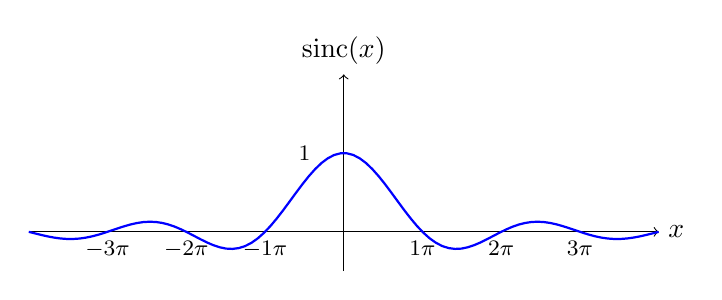
\begin{tikzpicture}[scale=1.0]
        % Asse x
        \draw[->] (-4,0) -- (4,0) node[right] {$x$};
        % Asse y
        \draw[->] (0,-0.5) -- (0,2) node[above] {$\operatorname{sinc}(x)$};

        % Grafico della funzione sinc
        \draw[thick, blue, domain=-4:4, samples=100] plot (\x, {sin(deg(pi*\x))/(pi*\x)});

        % Annotazioni per i punti significativi
        \foreach \x in {-3, -2, -1, 1, 2, 3} {
            \node[below] at (\x, 0) {\footnotesize $\x \pi$};
        }
        
        % Annotazioni sull'asse y
        \node[left] at (-0.3, 1) {\footnotesize $1$};
    \end{tikzpicture}
\end{center}
\end{definition}


\begin{definition}[Distribuzione impulso unitario - Delta di Dirac]
\(
    \begin{aligned}
        \delta(t)
        &= \lim_{T \rightarrow 0} \frac{1}{T} \Pi \left (\frac{t}{T} \right) \\
        &=
        \begin{cases}
            + \infty & \forall t=0 \\
            0
        \end{cases}
    \end{aligned}
\)

\begin{center}
    \begin{tikzpicture}[scale=1.0]
        % Asse x
        \draw[->] (-2,0) -- (2,0) node[right] {$t$};
        % Asse y
        \draw[->] (0,-0.5) -- (0,2) node[above] {$\delta(t)$};

        % Grafico della funzione delta
        \draw[thick, blue] (-2,0) -- (2,0); % Linea orizzontale

        % Freccia blu a t=0
        \draw[->, thick, blue] (0,0) -- (0,1)  node[midway,right]{\footnotesize $\infty$}; % Freccia verso l'alto
    \end{tikzpicture}
\end{center}

\begin{enumerate}[label=\roman*.]
    \item \(\forall \int_{-\infty}^{+\infty} f(t) \delta(t) dt = f(0)\)
    \item \(\int_{-\infty}^t \delta (t) dt = u(t)\)
\end{enumerate}
\end{definition}


\begin{definition}[Treno di impulsi]
    \(x(t)=\sum_{-\infty}^{\infty} \delta(t-kT)\)
\end{definition}


\subsection{Manipolazione dei segnali}

\begin{definition}[Traslazione temporale]
    \[\newline\]
    \begin{enumerate}[label=\roman*.]
        \item Ritardo \[x(t-\Delta t)\]
        \item Anticipo \[x(t+\Delta t)\]
    \end{enumerate}
\end{definition}

\begin{definition}[Riscalamento temporale]
    \[\newline\]
    \begin{enumerate}[label=\roman*.]
        \item Espansione \[x(kt) \hspace{1em} \forall k<1\]
        \item Compressione \[x(kt) \hspace{1em} \forall k>1\]
    \end{enumerate}
\end{definition}


\begin{definition}[Fattore di guadagno]
    \[\newline\]
    \begin{enumerate}[label=\roman*.]
        \item Amplificazione \[k x(t) \hspace{1em} \forall k>1\]
        \item Attenuazione \[k x(t) \hspace{1em} \forall k<1\]
    \end{enumerate}
\end{definition}

\begin{definition}[Derivazione]
    \[
        y(t)= \frac{d}{dt} x(t)
    \]
\end{definition}

\begin{definition}[Integrazione]
    \[
        y(t) = \int_{-\infty}^{t} x(t) dt
    \]
\end{definition}


\subsection{Statistiche dei segnali}

\begin{definition}[Valor medio]
    \[\newline\]
    \begin{enumerate}[label=\roman*.]
        \item \[<x(t)>_{(t_1,t_2)} = \frac{1}{\lvert t_2 - t_1 \rvert} \int_{t_1}^{t_2} x(t) dt\]
        \item \begin{align*}
                \overline x
                &= <x(t)> \\
                &= \lim_{T \rightarrow \infty} \frac{1}{T} \int_{-T/2}^{T/2} x(t) dt \end{align*}
    \end{enumerate}
\end{definition}

\begin{definition}[Valore quadratico medio]
    \begin{align*}
        \overline{x^2}
        &= <x(t)^2> \\
        &= \lim_{T \rightarrow \infty} \frac{1}{T} \int_{-T/2}^{T/2} x^2 (t) dt
    \end{align*}
\end{definition}

\begin{definition}[Varianza]
    \begin{align*}
        \sigma_x^2
        &= \overline{x^2} - x^{-2} \\
        &= \lim_{T \rightarrow \infty} \frac{1}{T} \int_{-T/2}^{T/2} (x(t) - \overline x)^2 dt
    \end{align*}
\end{definition}

\begin{definition}[Energia di un segnale]
    \[E_x = \int_{-\infty}^{+\infty} x^2 (t) dt \hspace{2em} [Watt]\]
\end{definition}

\begin{definition}[Potenza media di un segnale]
    \[P_x = \lim_{T \rightarrow \infty} \frac{1}{T} \int_{-T/2}^{T/2} x^2 (t) dt \hspace{2em} [Joule]\]
\end{definition}

\begin{definition}[Segnale di energia]
    \[
        \begin{cases}
            E_x = k \in \mathbb R \\
            P_x = 0
        \end{cases}
    \]
\end{definition}
\begin{definition}[Segnale di potenza]
    \[
        \begin{cases}
            E_x = \infty \\
            P_x = k \in \mathbb R
        \end{cases}
    \]
\end{definition}

\begin{definition}[Cross-correlazione]
    \[\newline\]
    \begin{enumerate}[label=\roman*.]
        \item Cross-correlazione tra segnali di energia
            \[R_{xy}(\tau)= \int_{-\infty}^{+\infty} x(t) y(t+\tau) dt\]
        \item Cross-correlazione tra segnali di potenza
            \[R_{xy}(\tau) = \lim_{T \rightarrow \infty} \frac{1}{T} \int_{-T/2}^{T/2} x(t)y(t+\tau) dt\]
    \end{enumerate}
\end{definition}

\begin{definition}[Autocorrelazione]
    \[\newline\]
    \begin{enumerate}[label=\roman*.]
        \item Autocorrelazione per segnali di energia
            \[R_{x}(\tau) = \int_{-\infty}^{+\infty} x(t) x(t+\tau) dt\]
        \item Autocorrelazione per segnali di potenza
            \[R_{x}(\tau) = \lim_{T \rightarrow \infty} \frac{1}{T} \int_{-T/2}^{T/2} x(t) x(t+\tau) dt\]
    \end{enumerate}
\end{definition}

\begin{proposition}[Proprietà dell'Autocorrelazione]
    \[\newline\]
    \begin{enumerate}[label=\roman*.]
        \item Segnali di potenza \[R_x (0) = \overline{x^2}\]
        \item Segnali di energia \[R_x (0) = E_x\]
    \end{enumerate}
\end{proposition}

\newpage


\section{Sistemi analogici}

\begin{definition}[Sistema]
    \[
        \overline{y}(\overline{v}) = \varphi (\overline{x}(\overline{u}))
    \]
\end{definition}

\subsection{Sistemi lineari tempo invarianti}

\begin{definition}[Sistemi LTI]
    \[
        y(t)=f(x(t))
    \]
\end{definition}

\begin{proposition}[Principio di sovrappozione degli effetti]
\[
    \begin{cases}
        f(x_1(t)) = y_1(t) \\
        f(x_2(t)) = y_2(t)
    \end{cases}
    \Rightarrow
    f(\alpha x_1(t) + \beta x_2(t)) = \alpha y_1 (t) + \beta y_2 (t)
\]
\end{proposition}

\begin{definition}[Tempo invarianza]
    \[f(x(t)) = y(t) \Rightarrow f(x(t-t_0)) = y(t-t_0)\]
\end{definition}

\subsection{Risposta dei sistemi LTI}

\begin{definition}[Integrale di convuluzione]
    \begin{align*}
        \lim_{\Delta t \rightarrow 0} y_R (t)
        &= \int_{-\infty}^{+\infty} x(\tau) h(t-\tau) d \tau \\
        &= y(t) \\
        &= x(t) * h(t)
    \end{align*}
\end{definition}

\begin{proposition}[Proprietà della convoluzione]
    \[\newline\]
    \begin{enumerate}[label=\roman*.]
        \item Proprietà commutativa della convoluzione \[x(t)*y(t)=y(t)*x(t)\]
        \item Proprietà associativa della convoluzione \[ x(t)*y(t)*z(t)= x(t)*[y(t)*z(t)] \]
        \item Proprietà distributiva della convoluzione \[x(t)*[y(t)+z(t)]=x(t)*y(t)+x(t)*z(t)\]
    \end{enumerate}    
\end{proposition}


\subsection{Convoluzioni notevoli}
\begin{proposition}[Convoluzione di impulsi]
    \[\newline\]
    \begin{enumerate}[label=\roman*.]
        \item \[x(t)*\delta(t) = x(t)\]
        \item \[x(t)*\delta(t-T)=x(t-T)\]
    \end{enumerate}
\end{proposition}


\begin{proposition}[Convoluzione di rettangoli simmetrici di pari durata]
        \(x_1(t) = A_1 \Pi (t/T) \)\\
        \(x_2(t) = A_2 \Pi (t/T)\)

        \[
        x_1(t)*x_2(t) =A_1 A_2 T \Lambda \left (\frac{t}{2T} \right)
        \]

        \begin{center}
            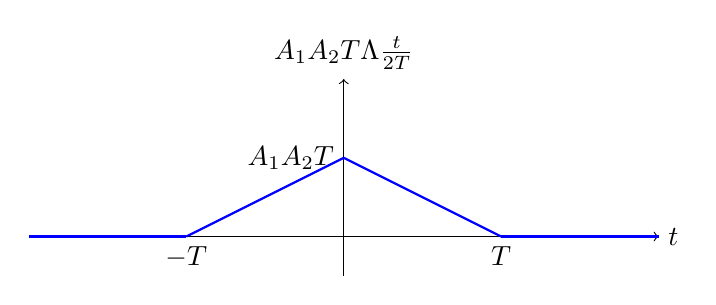
\begin{tikzpicture}
                % Asse x
                \draw[->] (-4,0) -- (4,0) node[right] {$t$};
                % Asse y
                \draw[->] (0,-0.5) -- (0,2) node[above] {$A_1 A_2 T \Lambda \frac{t}{2T}$};

                \draw[thick, blue] (-2,0) -- (0,1);
                \draw[thick, blue] (0,1) -- (2,0); 
                
                \draw[thick, blue] (-4,0)--(-2,0);
                \draw[thick, blue] (4,0)--(2,0);

                \node[left] at (0,1) {$A_1 A_2 T$};
                \node[below] at (-2,0) {$-T$};
                \node[below] at (2,0) {$T$};
            \end{tikzpicture}
        \end{center}
\end{proposition}


\begin{proposition}[Convoluzione di rettangoli simmetrici di diversa durata]
    \( \forall \,T_1<T_2\)

    \[
        y(t)= A_1A_2 \left( \frac{T_1+T_1}{2}-t \right)
    \]

    \begin{center}
        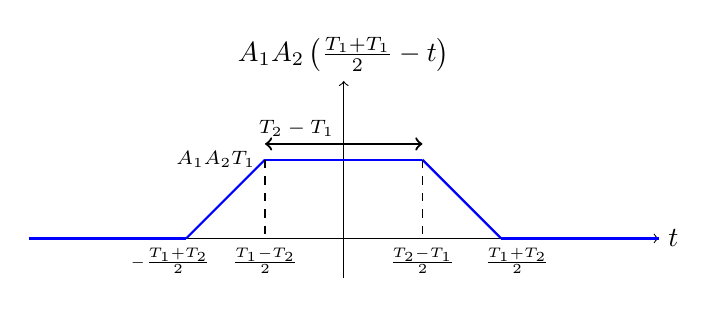
\begin{tikzpicture}
            % Asse x
            \draw[->] (-4,0) -- (4,0) node[right] {$t$};
            % Asse y
            \draw[->] (0,-0.5) -- (0,2) node[above] {$A_1A_2 \left( \frac{T_1+T_1}{2}-t \right)$};
        
            % Grafico della funzione rettangolo
            \draw[thick, blue] (-1, 1) -- (1, 1); 
            \draw[thick, blue] (1, 1) -- (2, 0);
            \draw[thick, blue] (-1, 1) -- (-2, 0);
            \draw[thick, blue] (2, 0) -- (4, 0);
            \draw[thick, blue] (-4, 0) -- (-2, 0);

            % Linea con doppia freccia
            \draw[<->, thick, black] (-1, 1.2) -- (1, 1.2);  
    
            % Linee tratteggiate
            \draw[dashed, black] (-1,1) -- (-1,0);
            \draw[dashed, black] (1,1) -- (1,0);
        
            % Annotazioni con testo ridotto
            \node[below, font=\tiny] at (-2.2, 0) {$-\frac{T_1 + T_2}{2}$};
            \node[below, font=\tiny] at (2.2, 0) {$\frac{T_1 + T_2}{2}$};
            \node[below, font=\tiny] at (-1, 0) {$\frac{T_1-T_2}{2}$};
            \node[below, font=\tiny] at (1, 0) {$\frac{T_2 -T_1}{2}$};
    
            \node[left, font=\scriptsize] at (0, 1.4) {$T_2 -T_1$};
            \node[left, font=\scriptsize] at (-1, 1) {$A_1 A_2 T_1$};
        \end{tikzpicture}
    \end{center}
    
\end{proposition}

\begin{proposition}[Convoluzione di rettangoli non simmetrici di pari durarta e ampiezza]
    \begin{align*}
        x_1(t)
        &= x_2(t) \\
        &=A \Pi \left ( \frac{t- T/2}{T} \right) \\
        &= A \Pi (t/T) * \delta ( t - T/2 )
    \end{align*}

    \begin{align*}
        x_1 (t) * x_2(t)
        &= A \Pi (t/T) * \delta ( t - T/2) * A \Pi (t/T) * \delta (t - T/2) \\
        &= A \Pi (t/T) * A \Pi (t/T)* \delta (t-T/2)*\delta(t-T/2) \\
        &= A^2 T \Lambda \left(\frac{t}{2T}\right) * \delta (t-T) \\
        &= A^2 T \Lambda \left(\frac{t-T}{2T}\right)
    \end{align*}

    \begin{center}
        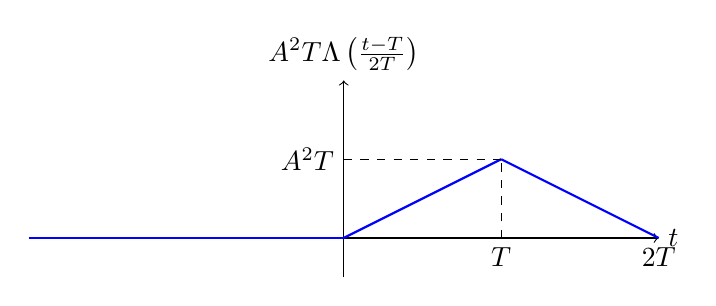
\begin{tikzpicture}
                % Asse x
                \draw[->] (-4,0) -- (4,0) node[right] {$t$};
                % Asse y
                \draw[->] (0,-0.5) -- (0,2) node[above] {$A^2 T \Lambda\left( \frac{t-T}{2T}\right)$};


                \draw[thick, blue] (0,0) -- (2,1);
                \draw[thick, blue] (2,1) -- (4,0); 
                
                \draw[thick, blue] (-4,0)--(0,0);
                \draw[dashed] (2,0)--(2,1);
                \draw[dashed] (0,1)--(2,1);

                \node[left] at (0,1) {$A^2 T$};
                \node[below] at (2,0) {$T$};
                \node[below] at (4,0) {$2T$};

            
        \end{tikzpicture}
    \end{center}
\end{proposition}

\begin{proposition}[Convoluzione di gaussiane]
    \(x_1(t) = \frac{1}{\sqrt{2\pi \sigma_1^2}} e^{- \frac{(t- \mu_1)^2}{2 \sigma_1^2}}\) \\
    \(x_2(t) = \frac{1}{\sqrt{2\pi \sigma_2^2}} e^{- \frac{(t- \mu_2)^2}{2 \sigma_2^2}}\)

    \[
        x_1(t)*x_2(t) = \frac{1}{\sqrt{2\pi (\sigma_1^2 + \sigma_2^2)}} e^{- \frac{[t- (\mu_1 + \mu_2)]^2}{2 (\sigma_2^2 + \sigma_2^2)}}
    \]

\end{proposition}

\begin{definition}[Causalità di un sistema in base alla risposta impulsiva]
    \(
        \forall t < 0
    \)
    \[
        h(t)=0
    \]    
\end{definition}

\newpage

\section{Serie di Fourier}

\subsection{Serie di Fourier}
\begin{definition}[Serie di Fourier]
    \begin{align*}
        x(t)
        &=a_0+\sum_{k=1}^{\infty} a_k \cos \left ( \frac{2 \pi k t}{T_0} + \theta_k\right) \\
        &= a_0 + \sum_{k=1}^\infty a_k \cos(2 \pi k f_0 t + \theta_k)
    \end{align*}
    
    \begin{enumerate}[label=\roman*.]
        \item \(f_0=\frac{1}{T_0}\) : frequenza fondamentale;
        \item \(a_k\) : armonica di ordine k;
        \item \(a_0\) : componente continua.
    \end{enumerate}
\end{definition}

\begin{definition}[Serie di Forurier in forma complessa]
    \( \forall \, \cos(2 \pi k f_0 t + \theta_k) = (e^{j(2\pi k f_0 t + \theta_k)}+e^{-j(2\pi k f_0 t + \theta_k)})/2\)

    \begin{align*}
        x(t)
        &= a_0 + \sum_{k=1}^{\infty} \frac{a_k}{2} e^{j \theta_k} e^{j2 \pi k f_0 t} + \sum_{k=1}^{\infty}  \frac{a_k}{2} e^{-j \theta_k} e^{-j2 \pi k f_0 t} \\
        &= a_0 + \sum_{k=1}^{\infty} a_k \cos(2\pi k f_0 t + \theta_k) \\
        &= a_0 + \sum_{k=1}^{\infty} a_k [e^{j(2\pi k f_0 t + \theta_k)}+e^{-j(2\pi k f_0 t + \theta_k)}]/2 \\
        &= a_0 + \sum_{k=1}^{\infty} \frac{a_k}{2} e^{j \theta_k} e^{j 2\pi k f_0 t} + \sum_{k=1}^{\infty} \frac{a_k}{2} e^{-j \theta_k} e^{-j 2 \pi k f_0 t} \\
        &=\sum_{k=-\infty}^{\infty}X_k e^{j2\pi k f_0 t}
    \end{align*}

    \begin{enumerate}[label=\roman*.]
        \item \(X_k\) : coefficienti complessi della serie di Fourier.
    \end{enumerate}

\end{definition}

\subsection{Coefficienti della serie di Fourier}

\begin{definition}[Coefficienti di Fourier]
    \begin{align*}
        X_k
        &=
            \begin{cases}
                \frac{a_k}{2} e^{j \theta_k} & k>0 \\
                \frac{a_{-k}}{2} e^{j \theta_{-k}} & k<0 \\
                a_0 & k=0
            \end{cases}  \\
        &= \frac{1}{T_0} \int_{-T_0/2}^{T_0/2} x(t) e^{-j2\pi k f_0 t} dt
    \end{align*}

    \begin{enumerate}[label=\roman*.]
        \item \(e^{-j 2 \pi k f_0 t}\) : sinusoide complessa - fasore;
        \item \(X_k\) equivale alla cross-correlazione per segnali di potenza tra il segnale \(x(t)\) ed il fasore \(e^{-j 2 \pi k f_0 t}\) calcolato nell'origine.
    \end{enumerate}
\end{definition}

\begin{definition}[Coefficienti di Fourier per k=0]
    \[X_0 = \frac{1}{T_0} \int_{-T_0/2}^{T_0/2} x(t) \, dt\]

    \begin{enumerate}[label=\roman*.]
        \item \(X_0\) equivale al valor medio di \(x(t)\).
    \end{enumerate}
\end{definition}

\subsection{Proprietà della serie di Fourier}

\begin{proposition}[Proprietà della serie di Fourier]
    \[\newline\]
    \begin{enumerate}[label=\roman*.]
        \item Simmetria Hermitiana 
        \[
        X_n = -X^*_{-n} \Leftrightarrow 
        \begin{cases}
            \lvert X_n \rvert = \lvert X_{-n} \rvert \\
            \arg (X_n) = -\arg (X_{-n})
        \end{cases}
        \]
        \item Linearità
        \[
            z(t)=\alpha x(t) \beta y(t) \Rightarrow Z_k =\alpha X_k + \beta Y_k
        \]
        \item Segnale pari \[X_k = \frac{2}{T_0} \int_{0}^{T_0/2} x(t) \cos(2\pi k f_0 t) dt\]
        \item Segnale dispari \[X_k = -\frac{2j}{T_0} \int_{0}^{T_0/2} x(t) \sin(2 \pi k f_0 t) dt\]
    \end{enumerate}
\end{proposition}

\subsection{Coefficienti di forme d'onda notevoli}
\begin{proposition}[Onda quadra]
    \begin{center}
        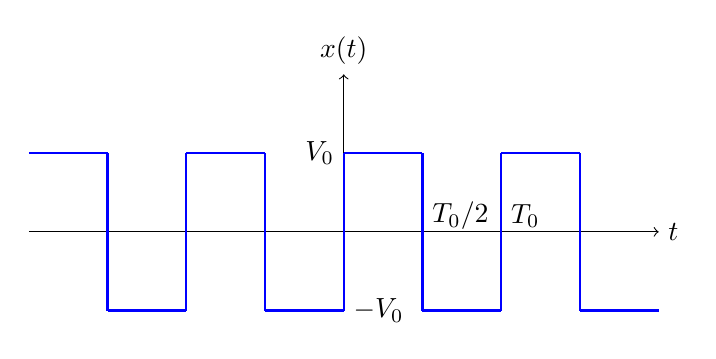
\begin{tikzpicture}
            % Asse x
            \draw[->] (-4,0) -- (4,0) node[right] {$t$};
            % Asse y
            \draw[->] (0,-0.5) -- (0,2) node[above] {$x(t)$};

            \draw[thick, blue] (-4,1)--(-3,1);
            \draw[thick, blue] (-3,1)--(-3,-1);
            \draw[thick, blue] (-3,-1)--(-2,-1);
            \draw[thick, blue] (-2,-1)--(-2,1);
            \draw[thick, blue] (-2,1)--(-1,1);
            \draw[thick, blue] (-1,1)--(-1,-1);
            \draw[thick,blue] (-1,-1)--(0,-1);
            \draw[thick, blue] (0,-1)--(0,1);

            \draw[thick, blue] (0,1)--(1,1);
            \draw[thick, blue] (1,1)--(1,-1);
            \draw[thick, blue] (1,-1)--(2,-1);
            \draw[thick, blue] (2,-1)--(2,1);
            \draw[thick, blue] (2,1)--(3,1);
            \draw[thick, blue] (3,1)--(3,-1);
            \draw[thick,blue] (3,-1)--(4,-1);

            \node[left] at (0,1) {$V_0$};
            \node[right] at (0,-1) {$-V_0$};

            \node[right] at(1,0.2) {$T_0/2$};
            \node[right] at(2,0.2) {$T_0$};
        \end{tikzpicture}
    \end{center}

    \begin{align*}
        X_k
        &= -\frac{2j}{T_0} \int_{0}^{T_0/2} x(t) \sin(2 \pi k f_0 t) dt \\
        &= - \frac{2j}{T_0} \int_{0}^{T_0 /2} V_0 \sin (2 \pi k f_0 t) dt \\
        &=  \left [j \frac{2 V_0 \cos (2 \pi k f_0 t)}{2 \pi k f_0 T_0} \right]_{0}^{T_0/2} \\
        &= \frac{j V_0}{\pi k} [\cos(\pi k) - 1] \\
        &= \frac{j V_0}{\pi k} [(-1)^k -1] \\
        &=
            \begin{cases}
                0 & k \, pari \\
                \frac{-2jV_0}{\pi k} & k \, dispari
            \end{cases}
    \end{align*}
\end{proposition}

\begin{proposition}[Onda quadra con ritorno a zero]

    \begin{center}
        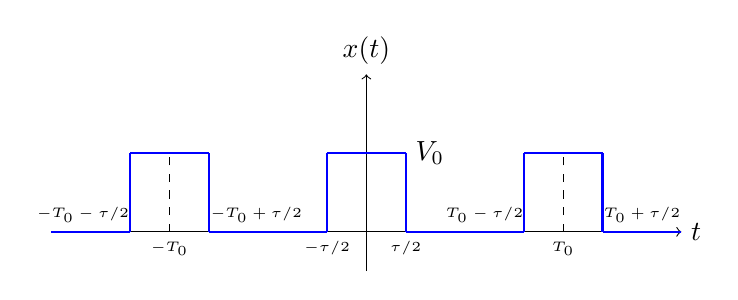
\begin{tikzpicture}
            % Asse x
            \draw[->] (-4,0) -- (4,0) node[right] {$t$};
            % Asse y
            \draw[->] (0,-0.5) -- (0,2) node[above] {$x(t)$};

            \draw[thick, blue] (-4,0)--(-3,0);
            \draw[thick, blue] (-3,0)--(-3,1);
            \draw[thick, blue] (-3,1)--(-2,1);
            \draw[thick, blue] (-2,1)--(-2,0);
            \draw[thick, blue] (-2.,0)--(-0.5,0);
            \draw[thick, blue] (-0.5,0)--(-0.5,1);
            \draw[thick, blue] (-0.5,1)--(0.5,1);

            \draw[thick, blue] (4,0)--(3,0);
            \draw[thick, blue] (3,0)--(3,1);
            \draw[thick, blue] (3,1)--(2,1);
            \draw[thick, blue] (2,1)--(2,0);
            \draw[thick, blue] (2.,0)--(0.5,0);
            \draw[thick, blue] (0.5,0)--(0.5,1);

            \node[below, font=\tiny] at(-0.5,0) {$-\tau/2$};
            \node[below, font=\tiny] at(0.5,0) {$\tau/2$};

            \node[above, font=\tiny] at(-1.4,0) {$-T_0 + \tau/2$};
            \node[above, font=\tiny] at(-3.6,0) {$-T_0 - \tau/2$};
            \node[below, font=\tiny] at(-2.5,0) {$-T_0$};

            \node[above, font=\tiny] at(1.5,0) {$T_0 - \tau/2$};
            \node[above, font=\tiny] at(3.5,0) {$T_0 + \tau/2$};
            \node[below, font=\tiny] at(2.5,0) {$T_0$};

            \draw[dashed] (-2.5,0)--(-2.5,1);
            \draw[dashed] (2.5,0)--(2.5,1);

            \node[right] at (0.5,1) {$V_0$};
        \end{tikzpicture}
    \end{center}

    \begin{align*}
        X_k
        &= \frac{2}{T_0} \int_{0}^{T_0/2} x(t) \cos(2\pi k f_0 t) dt \\
        &= \frac{2}{T_0} \int_{0}^{\tau/2} V_0 \cos(2 \pi k f_0 t) dt \\
        &= \left [\frac{2V_0 \sin(2 \pi k f_0 t)}{T_0 2 \pi k f_0} \right]_{0}^{\tau/2} \\
        &= \frac{V_0 \tau \sin(\pi k f_0 \tau)}{T_0 \pi k f_0 \tau} \\
        & \frac{V_0 \tau}{T_0} \operatorname{sinc}(k f_0 \tau)
    \end{align*}
    
    \begin{enumerate}[label=\roman*.]
        \item \(\tau/T_0\) : duty cycle.
    \end{enumerate}
\end{proposition}


\begin{proposition}[Onda triangolare]
    \begin{center}
        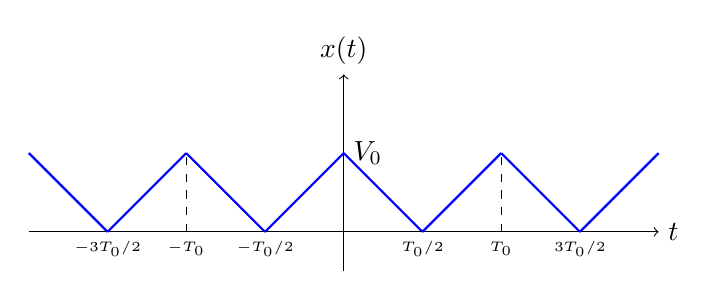
\begin{tikzpicture}
            % Asse x
            \draw[->] (-4,0) -- (4,0) node[right] {$t$};
            % Asse y
            \draw[->] (0,-0.5) -- (0,2) node[above] {$x(t)$};

            \draw[thick, blue] (-4,1)--(-3,0);
            \draw[thick, blue] (-3,0)--(-2,1);
            \draw[thick, blue] (-2,1)--(-1,0);
            \draw[thick, blue] (-1,0)--(0,1);


            \draw[thick, blue] (4,1)--(3,0);
            \draw[thick, blue] (3,0)--(2,1);
            \draw[thick, blue] (2,1)--(1,0);
            \draw[thick, blue] (1,0)--(0,1);

            \node[right] at(0,1) {$V_0$};
            
            \node[below, font=\tiny] at(-3,0) {$-3T_0/2$};
            \node[below, font=\tiny] at(-1,0) {$-T_0/2$};

            \node[below, font=\tiny] at(1,0) {$T_0/2$};
            \node[below, font=\tiny] at(3,0) {$3T_0 / 2$};

            \node[below, font=\tiny] at(-2,0) {$-T_0$};
            \node[below, font=\tiny] at (2,0) {$T_0$};

            \draw[dashed] (2,0)--(2,1);
            \draw[dashed] (-2,0)--(-2,1);

            \draw[thick, blue];
        \end{tikzpicture}
    \end{center}

    \begin{align*}
        X_K
        &= \frac{2V_0}{T_0} \int_{0}^{T_0/2} x(t) \cos (2 \pi k f_0 t) dt \\
        &= \frac{2V_0}{T_0} \int_{0}^{T_0/2} \left ( 1 - \frac{2V_0}{T_0}  \cos(2 \pi k f_0 t) dt \right ) \\
        &= \frac{2V_0}{T_0} \int_{0}^{T_0/2} \cos (2 \pi k f_0 t) dt - \frac{4 V_0}{T_0 ^2} \int_{0}^{T_0/2} t \cos (2 \pi k f_0 t) dt \\
        &= \frac{4V_0}{T_0^2} \left [ \frac{t}{2\pi k f_0} \sin(2 \pi k f_0 t) \Big |_{0}^{T_0/2} - \frac{1}{2 \pi k f_0} \int_{0}^{T_0/2} \sin (2 \pi k f_0 t) dt \right] \\
        &= \frac{4 V_0}{T_0 ^2 (2 \pi k f_0)^2} [1- \cos (\pi k)] \\
        &= \frac{8 V_0}{T_0 ^2 (2 \pi k f_0)^2} \sin^2 (\pi k /2) \\
        &= \frac{2 V_0}{(\pi k)^2} \sin^2 (\pi k/2) \\
        &= \frac{V_0 \sin^2 (\pi k /2)}{2 (\pi k/2)^2} \\
        &= \frac{V_0}{2} \operatorname{sinc}^2 (k/2)
    \end{align*}
\end{proposition}


\begin{theorem}[Teorema di Parseval]
    \begin{align*}
        P_x
        &= \frac{1}{T} \int_{0}^{T} x^2 (t) dt \\
        &= \frac{1}{T} \int_{0}^{T} \left\{ \sum_{n=-\infty}^{\infty} X_k e^{j2 \pi n f_0 t}  \cdot \sum_{k=-\infty}^{\infty} X_k e^{j 2 \pi k f_0 t} \right\} dt \\
        &= \frac{1}{T} \sum_{n=-\infty}^{\infty} \sum_{k=-\infty}^{\infty} X_n X_k \int_{0}^{T} e^{j2 \pi (n+k)f_0 t} dt \\
        &= \frac{1}{T} \sum_{n=-\infty}^{\infty} \sum_{k=-\infty}^{\infty} X_n X_{-n} \\
        &= \sum_{k=-\infty}^{+\infty} \lvert X_n \rvert ^2
    \end{align*}

    \begin{enumerate}[label=\roman*.]
        \item
           \(\int_{0}^{T} e^{j 2 \pi (n+k) f_0 t} dt =
           \begin{cases}
            T & n+k=0 \\
            0
           \end{cases}\)
        \item La potenza media del segnale è pari alla somma delle potenze delle singole armoniche.
    \end{enumerate}
\end{theorem}

\newpage

\section{Trasformata di Fourier}

\subsection{Dalla serie alla Trasformata di Fourier}

\(x(t) = \sum_{k=-\infty}^{\infty} \Pi \left( \frac{t- kT_0}{\tau} \right) \leftrightarrow x_k = \frac{\tau}{T_0} \operatorname{sinc} (k f_0 \tau)\)

\(\forall \, \lim_{T_0 \to \infty} \{x(t)\} = w(t)\)

\begin{align*}
    x(t)
    &= \sum_{k=-\infty}^{\infty} w(t-kT_0) \\
    &= w(t) * \sum_{k=-\infty}^{\infty} \delta(t - k T_0)
\end{align*}

\begin{definition}[Coefficiente di Fourier modificato]
    \begin{align*}
        X(k f_0)
        &= T_0 X_k \\
        & \int_{-T_0 /2}^{T_0/2} w(t) e^{-j 2 \pi k f_0 t} dt
    \end{align*}
\end{definition}

\begin{definition}[Serie di Fourier modificata]
    \[x(t) = \sum_{k=-\infty}^{\infty} X(k f_0) e^{j 2 \pi k f_0 t} f_0\]
\end{definition}

\begin{align*}
    \lim_{T_0 \to \infty} x(t) 
    &= w(t) \\
    &= \lim_{f_0 \to 0} \sum_{k=-\infty}^{\infty} X(k f_0) e^{j 2 \pi k f_0 t} f_0 \\
    &= \int_{-\infty}^{\infty} X(f) e^{j2 \pi f t} df
\end{align*}


\begin{align*}
    X(f)
    &= \lim_{f_0 \to 0} X(k f_0) \\
    &= \lim_{\substack{T_0 \to \infty \\ f_0 \to 0}} \int_{-T_0 /2}^{T_0 /2} w(t) e^{-2 \pi j k f_0 t} dt \\
    &= \int_{-\infty}^{\infty} w(t) e^{-j2 \pi f t} dt
\end{align*}

\subsection{Trasformata di Fourier}
\begin{definition}[Trasformata di Fourier - Rappresentazione in frequenza]
    \[
        X(f) = \int_{-\infty}^{+\infty} w(t) e^{-j2\pi f t} dt
    \]
\end{definition}

\begin{definition}[Antitrasformata di Fourier- Ricostruzione nel tempo]
    \[
        w(t) = \int_{-\infty}^{+\infty} X(f) e^{j 2 \pi f t} df
    \]
\end{definition}

\begin{definition}[Coppia di Fourier]
    \[x(t) \leftrightarrow X(f)\]
\end{definition}

\subsection{Proprietà della trasformata di Fourier}

\begin{proposition}[Proprietà della trasformata di Fourier]
    \[\newline\]
    \begin{enumerate}[label=\roman*.]
        \item Simmetria Hermitiana
            \[x(t) \in \mathbb R \Rightarrow X(f) = X^* (-f)\]
                \[\Leftrightarrow\]
            \[    \begin{cases}
                    \Re \{X(f)\} = \Re \{X(-f)\} \\
                    \Im \{X(f)\} = - \Im \{X(-f)\} \\
                    \lvert X(f) \rvert = \lvert X(-f) \rvert \\
                    \arg\{X(f)\} = - \arg\{X(-f)\}
                \end{cases}
            \]
        \item Simmetria del segnale nel tempo
            \[
                x(-t)=x(t) \Rightarrow X(f)= 2 \int_{0}^{+\infty} x(t) \cos(2\pi ft) dt
            \]
            \[
                x(-t) = -x(t)\Rightarrow X(f)= -2j \int_{0}^{+\infty} x(t) \sin(2\pi ft) dt
            \]
        \item Linearità
            \[
                \begin{cases}
                    x(t) \leftrightarrow X(f) \\
                    y(t) \leftrightarrow Y(f)
                \end{cases}
                \Rightarrow \alpha x(t) + \beta y(t) \leftrightarrow a X (f) + \beta Y(f)
            \]

        \item Fattore di scala
            \[x(t) \leftrightarrow X(f) \Rightarrow x (\alpha t) \leftrightarrow \frac{1}{\alpha} X \left(\frac{f}{\alpha} \right)\]
        \item Traslazione
            \[ x (t) \leftrightarrow X(f) \Rightarrow x(t-T) \leftrightarrow X(f) e^{-j 2 \pi fT}\]
        \item Dualità
            \[x(t) \rightarrow X(f) \Leftrightarrow X(t) \rightarrow x(-f)\]
        \item Derivazione
            \[y(t) =\frac{d}{dx} x(t) \leftrightarrow Y(f) = j 2 \pi f \cdot X(f)\]
        \item Integrazione
            \[x(t) \leftrightarrow X(f) \Rightarrow \int_{-\infty}^{t} x(\zeta) d \zeta \leftrightarrow \frac{X(f)}{j2 \pi f} + \frac{X(0)}{2} \delta (f)\]
        \item Convoluzione
            \[
                \begin{cases}
                    x(t) \leftrightarrow X(f) \\
                    y(t) \leftrightarrow Y(f)
                \end{cases}
                \Rightarrow x(t) * y(t) = X(f) \cdot Y(f)
            \]

        \item Prodotto
            \[
                \begin{cases}
                    x_1 (t) \leftrightarrow X_1(f) \\
                    x_2 (t) \leftrightarrow X_2(f)
                \end{cases}
                \Rightarrow x_1 (t) \cdot x_2 (t) \leftrightarrow X_1(f)*X_2(f)
            \]
        \item Modulazione
        \begin{align*}
            X(f) &= 
            M(f) * \frac{1}{2} \left[ \delta(f-f_0) + \delta(f+f_0) \right] \\
            &= \frac{1}{2} \left[ M(f-f_0) + M(f+f_0) \right]
        \end{align*}
    \end{enumerate}
\end{proposition}

\subsection{Trasformate notevoli}

\begin{proposition}[Rettangolo]
    \begin{align*}
        x(t) = V_0 \Pi (t/T) \rightarrow X(f)
        &= \int_{-T/2}^{T/2} V_0 e^{-2 \pi j f t} dt \\
        &= \frac{V_0}{2 \pi j f} [e^{\pi jfT}-e^{-\pi jfT}] \\
        &= \frac{V_0 T [e^{\pi jfT}-e^{-\pi jfT}]}{2\pi jfT} \\
        &= V_0 T \frac{\sin(\pi fT)}{\pi f T}\\
        &= V_0 T \operatorname{sinc}(fT)
    \end{align*}
\end{proposition}

\begin{proposition}[Costante]
    \begin{align*}
        x(t) = V_0 \Pi (t/T) \rightarrow X(f)
        &= V_0 T \operatorname{sinc} (fT) \\
        &\Rightarrow \lim_{T \rightarrow \infty} V_0 \Pi (t/T) =V_0 \rightarrow V_0 \delta (f)
    \end{align*}
\end{proposition}

\begin{proposition}[Esponenziale causale]
    \(\forall \alpha >0\)

    \begin{align*}
        x(t)= e^{-\alpha t} \cdot 1(t) \rightarrow X(f)
        &= \int_{0}^{\infty} e^{-\alpha t} \cdot e^{-j2 \pi ft} dt \\
        &= \int_{0}^{\infty} e^{-(\alpha + j2 \pi f)t} dt \\
        &= -\frac{[e^{-(\alpha + j2 \pi f)t}]_{0}^{\infty}}{\alpha + j2 \pi f} \\
        &= \frac{1}{\alpha + j2 \pi f}
    \end{align*}
\end{proposition}

\begin{proposition}
    \[\newline\]
    \begin{enumerate}[label=\roman*.]
        \item \[\mathcal{F}[\cos(2 \pi f_0 t)] = \frac{1}{2} [\delta (f+f_0)+\delta(f-f_0)]\]
        \item \[\mathcal{F}[ \sin(2 \pi f_0 t)] = \frac{j}{2} [\delta(f+f_0)-\delta(f-f_0)]\]
    \end{enumerate}
\end{proposition}

\begin{proposition}[\(\delta\) di Dirac]
    \[\newline\]
    \begin{enumerate}[label=\roman*.]
        \item \[\delta (t) \rightarrow 1\]
        \item \[\delta(t-\Delta T) \rightarrow e^{-j 2 \pi f \Delta T}\]
        \item \[\delta ' (t- \Delta T) \rightarrow j 2 \pi f e^{-j 2 \pi f \Delta T}\]
    \end{enumerate}
\end{proposition}

\begin{proposition}[Gradino unitario]
    \[
        1(t) \rightarrow \frac{1}{j2\pi f} + \frac{1}{2} \delta (f)
    \]
\end{proposition}

\begin{proposition}
    \[
        A f_0 \int_{-\infty}^{t} \sin(f_0 \zeta) d\zeta \rightarrow \frac{A \pi (f/f_0)}{j2 \pi f} + \frac{A}{2} \delta (f)
    \]
\end{proposition}

\begin{proposition}[Seno cardinale]
    \[
        A \operatorname{sinc} (\alpha t) \rightarrow \frac{A}{\alpha} \Pi (f/\alpha)
    \]
\end{proposition}

\begin{proposition}[Trasformate notevoli]
    \[\newline\]
    \begin{enumerate}[label=\roman*.]
    \item    \[
        \mathcal{F}\left[V_0 \Pi \left(\frac{t}{T}\right)\right] = V_0 T \operatorname{sinc}(fT)
        \]
    \item    \[
        \mathcal{F}[V_0 ]= V_0 \delta (f)
        \]
    \item    \[
        \mathcal{F}[e^{- \alpha t}]  = \frac{1}{\alpha + j2 \pi f}
        \]
    \item    \[
        \mathcal{F}[\cos(2 \pi f_0 t)] = \frac{1}{2} [\delta (f+f_0)+\delta(f-f_0)]
        \]
    \item    \[
        \mathcal{F}[ \sin(2 \pi f_0 t)] = \frac{j}{2} [\delta(f+f_0)-\delta(f-f_0)]
        \]
\end{enumerate}
\end{proposition}

\subsection{Trasformata di Fourier di segnali periodici}

\begin{definition}[Rappresentazione alternativa del generico segnale periodico]
        \begin{align*}
            x(t)
            &= \sum_{-\infty}^{+\infty} w(t - \eta T)\\
            &= w(t) * \sum_{-\infty}^{+\infty} \delta (t - \eta T)
        \end{align*}
\end{definition}

\begin{definition}[Trasformata di Fourier di segnali periodici]
    \begin{align*}
        X(f)
        &= W(f) \frac{1}{T} \sum_{k=-\infty}^{+\infty} \delta (f- k/T) \\
        &= \sum_{k=-\infty}^{+\infty} \frac{1}{T} W(K/T) \delta(f-k/T)
    \end{align*}
\end{definition}

\subsection{Energia nel dominio delle frequenze}
\begin{theorem}[Teorema di Rayleigh]
    \begin{align*}
        E_x
        &= \int_{-\infty}^{+\infty} \lvert x(t) \rvert^2 dt \\
        &= \int_{-\infty}^{+\infty} \lvert X(f) \rvert ^2 df
    \end{align*}
\end{theorem}

\begin{definition}[Densità spettrale di energia]
    \[E(f) = \lvert X(f) \rvert ^2\]
\end{definition}

\end{multicols}

\newpage

\section{Sistemi analogici in frequenza}
\subsection{Risposta in frequenza}
\begin{definition}[Risposta impulsiva]
    \(y(t) = x(t)*h(t) \leftrightarrow Y(f) = X(f) \cdot H(f)\)
    \[
        H(f)  = \frac{Y(f)}{X(f)}
    \]
\end{definition}

\begin{definition}[Risposta in frequenza ad un fasore]
    \(x(t) = e^{j2 \pi f_0 t}\)
    \[
        \begin{aligned}
            y(t)
            &= x(t) *h(t)   \\
            &= \int_{-\infty}^{+\infty} h(\zeta) e^{j 2 \pi f_0 (t-\zeta)} d \zeta \\
            &= e^{j2 \pi f_0 t} \int_{-\infty}^{+\infty} h(\zeta) e^{-j2 \pi f_0 \zeta} d\zeta \\
            &= x(t) \int_{-\infty}^{+\infty} h(\zeta) e^{-j 2 \pi f_0 \zeta} d\zeta \\
            \Rightarrow \frac{y(t)}{x(t)}
            &= \int_{-\infty}^{+\infty} h(\zeta) e^{-j 2 \pi f_0 \zeta} d \zeta \\
            &= \mathcal{F}\{h(t)\} \rvert_{f=f_0}   \\
            &= H(f_0)
        \end{aligned}
    \]
\end{definition}

\begin{definition}[Risposta in ampiezza]
    \[
        \lvert H(f) \rvert
    \]
\end{definition}

\begin{definition}[Risposta in fase]
    \[
        \Phi (f) = \arg [H(f)]
    \]
\end{definition}

\begin{definition}[Ritardo di gruppo]
    \[
        \tau(f) = - \frac{1}{2 \pi} \cdot  \frac{d}{df} \Phi(f)
    \]
\end{definition}

\subsection{Composizione di funzioni di trasferimento}

\begin{definition}[Sequenza]
    \[
    \begin{aligned}
        Y(f)
        &= [X(f) \cdot H_1(f)] \cdot H_2(f) \\
        &= X(f) \cdot [H_1 (f) \cdot H_2 (f)] \\
    \end{aligned}
    \]
    \[
    \begin{aligned}
        \Rightarrow H_{eq} (f)
        &= \frac{Y(f)}{X(f)} \\
        &= H_1 (f) \cdot H_2 (f)
    \end{aligned}
    \]
\end{definition}

\begin{definition}[Parallelo]
    \[
        \begin{aligned}
            Y(f)
            &= X(f) \cdot H_1 (f) \pm X(f) \cdot H_2 (f) \\
            &= X(f) \cdot [H_1 (f) \pm H_2 (f)]
        \end{aligned}
    \]

    \[
        \begin{aligned}
            H_{eq} (f)
            &= \frac{Y(f)}{X(f)} \\
            &= H_1 (f) \pm H_2 (f)
        \end{aligned}
    \]
\end{definition}

\begin{definition}[Retroazione negativa]
    \[
        \begin{aligned}
            Y(f)
            &= [X(f) -Y(f) \cdot H_2 (f)] \cdot H_1(f) \\
            &= X(f) \cdot H_1 (f) - Y(f) \cdot H_1 (f) \cdot H_2 (f)
        \end{aligned}
    \]

    \[
        \begin{aligned}
            \Rightarrow Y(f) [1 + H_1 (f) \cdot H-2 (f)] 
            &= X(f) \cdot H_1(f)
        \end{aligned}
    \]

    \[
        \begin{aligned}
            \Rightarrow H_{eq} (f)
            &= \frac{Y(f)}{X(f)} \\
            &= \frac{H_1 (f)}{1 + H_1 (f) \cdot H_2 (f)}
        \end{aligned}
    \]
\end{definition}

\subsection{Banda passante di un sistema LTI}
\begin{definition}[Guadagno di un sistema in funzione della frequenza]
    \[G(f) = \lvert H(f) \rvert\]
\end{definition}

\begin{definition}[Banda passante]
    \(\forall \, G_{dB} = 10 \log_{10} G = -3 dB \Rightarrow G= 10^{-\frac{3}{10}} \approx \frac{1}{2}\)
    \[B=f_{max} : G_{dB} (f_{max}) \geq -3 dB\]
\end{definition}

\subsection{Filtri LTI}

\begin{definition}[Risposta di un filtro ideale]
    \[H(f) =
    \begin{cases}
        ke^{-j2 \pi f t d} & f_1<f<f_2\\
        0
    \end{cases}\]
\end{definition}

\begin{definition}[Filtro passa-tutto (APF)]
    \[
        \begin{cases}
            f_1=0 \\
            f_2= \infty
        \end{cases}
    \]
\end{definition}

\begin{definition}[Filtro passa-basso (LPF)]
    \[
    \lvert f \rvert < f_2 \Leftrightarrow
        \begin{cases}
            f_1=0   \\
            f_2>0
        \end{cases}
    \]
\end{definition}

\begin{definition}[Filtro passa-alto (HPF)]
    \[
    \lvert f \rvert > f_1 \Leftrightarrow
        \begin{cases}
            f_1>0 \\
            f_2= \infty
        \end{cases}
    \]
\end{definition}

\begin{definition}[Filtro passa-banda (BPF)]
    \[
        f_1 < \lvert f \rvert f_2 \Leftrightarrow
    \]
\end{definition}

\begin{definition}[Filtro non causale]
    \(\forall \, t<0\)
    \[
        h(t) \neq 0
    \]    
\end{definition}

\begin{definition}[Regola della banda frazionaria]
    \[B=\frac{\Delta f}{f_1}\]
\end{definition}

\begin{definition}[Analizzatore di spettro]
    \(
        \begin{aligned}
            X(f)
            &= X_1 (f) + \ldots + X_n (f)   \\
            &= X(f) H_0 (f) + \ldots + X(f) H_n (f)
        \end{aligned}
    \)

    \[
        \begin{aligned}
            E_x 
            &= \int_{-\infty}^{+\infty} x^2 (t) dt \\
            &= \int_{-\infty}^{+\infty} X^2 (f) df \\
            &=\int_{-\infty}^{+\infty} X_0^2 (f) df + \ldots + \int_{-\infty}^{+\infty} X_n^2 (f) df \\
            &=2\int_{0}^{f_0} X^2 (f) df + 2 \int_{f_0}^{f_1} X^2(f) df + \ldots + 2 \int_{f_{n-1}}^{\infty} X^2 (f) df \\
            &= E_0 + \ldots + E_n
        \end{aligned}
    \]
\end{definition}


\newpage

\section{Distorsione e equalizzazione}

\subsection{Sistemi non distorcenti}
\begin{definition}[Canale ideale]
    \[H_{ci}(f) = k e^{-j 2 \pi f t_0}\]
\end{definition}

\subsection{Distorsione lineare}

\subsection{Equalizzazione}
\begin{definition}[Equalizzazione]
    \[
        \begin{aligned}
            H_{TOT}(f)
            &=H_S (f) \cdot H_{EQ}(f)   \\
            &=ke^{-j2\pi f t_0} \\
            \Rightarrow
            H_{EQ} (f)
            &= \frac{H_{TOT}(f)}{H_S(f)}    \\
            &= \frac{k e^{-j 2 \pi f t_0}}{H_S(f)}
        \end{aligned}
    \]
\end{definition}

\begin{definition}[Distorsione multi-path]
    
\end{definition}

\subsection{Distorsioni non lineari}


\newpage

\section{Conversione AD-DA}

\subsection{Campionamento ideale}
\begin{definition}[Campione ideale]
    \(\forall \, T_c : periodo \, di\,  campionamento\)
    \[
        x[n] = x(nT_c)
    \]
\end{definition}

\begin{definition}[Campionamento ideale]
    \[
        \begin{aligned}
            x_c(t)
            &=x(t) \sum_{n=-\infty}^{+\infty} \delta (t-nT_c) \\
            &=\sum_{n=-\infty}^{+\infty} x(nT_c) \delta (t-nT_c)
        \end{aligned}
    \]
\end{definition}

\subsection{Spettro del segnale campionato}
\begin{definition}[Spettro del segnale campionato]
    \[
        \begin{aligned}
            X_c(f)
            &= X(f) * \frac{1}{T_c} \sum_{k=-\infty}^{+\infty} \delta (f-kf_c)  \\
            &= \frac{1}{T_c} \sum_{k=-\infty}^{+\infty} X(f-kf_c)
        \end{aligned}
    \]
\end{definition}

\subsection{Teorema del campionamento}
\begin{theorem}[Condizione di Nyquist]
    \[f_c \geq 2 f_{max}\]
\end{theorem}

\begin{definition}[Sovracampionamento]
    \(\forall \, \epsilon : \, banda\,di\,guardia\)
    \[f_c = 2 f_{max} + \epsilon\]
\end{definition}

\subsection{Ricostruzione del segnale continuo}

\subsection{Interpolazione dei campioni}

\subsection{Sample and Hold}
\begin{definition}[Sample and Hold]
    \(
        x_{sh}(t)=x_c(t)*h_H(t)\\
        \Rightarrow X_{sh}(f) = X_C(f) \cdot H_H (f)
    \)
    \[
        H_{eq}(f) =
        \begin{cases}
            \frac{1}{H_H(f)} & \lvert f \rvert < f_{max} \\
            0    
        \end{cases}
    \]
\end{definition}

\subsection{Quantizzazione}
\begin{definition}[Quantizzazione]
    \(\forall
    \begin{cases}
        x(nT_c) & segnale \, campionato \\
        x_q(nT_c) & segnale \, quantizzato \\
        \epsilon_q(nT_c) & errore \, di \, quantizzazione
    \end{cases}\)
    \[x(nT_c)=x_q(nT_c)+\epsilon_q(nT_c)\]
\end{definition}

\begin{definition}[Quantizzatore uniforme]
    \[\Delta = \frac{2}{M} \Rightarrow \lvert \epsilon_{q_{max}} \rvert = \frac{\Delta}{2}= \frac{1}{M}\]
\end{definition}

\subsection{Rumore di quantizzazione}
\begin{definition}[Rumore di quantizzazione]
    \[
        \begin{aligned}
            E\{\epsilon_q^2\}
            &= \sigma_q^2 \\
            &= \int_{-\frac{\Delta}{2}}^{\frac{\Delta}{2}} \epsilon^2 f_{\epsilon_q} (\epsilon) d\epsilon \\
            &= \frac{1}{\Delta} \int_{-\frac{\Delta}{2}}^{\frac{\Delta}{2}} \epsilon^2 d \epsilon \\
            &= \frac{1}{\Delta} \frac{\epsilon ^3}{3} \rvert_{-\frac{\Delta}{2}}^{\frac{\Delta}{2}} \\
            &= \frac{\Delta ^2}{12}
        \end{aligned}
    \]
\end{definition}

\subsection{Rapporto segnale-rumore}
\begin{definition}[Rapporto segnale-rumore]
    \[
        \begin{aligned}
            SNR = 10 \log_{10} \frac{S_x}{S_n} \hspace{1em} [dB]
        \end{aligned}
    \]
\end{definition}

\begin{definition}[Segnale-Rumore del quantizzatore uniforme]
    \(
        \begin{aligned}
            E\{x^2\}
            &= \sigma_x^2 \\
            &= \int_{-\frac{A}{2}}^{\frac{A}{2}} x^2 f_x(x) dx \\
            &= \frac{1}{A} \int_{-\frac{A}{2}}^{\frac{A}{2}} x^2 dx \\
            &= \frac{A^2}{12} \\
            \Rightarrow \frac{S}{N}
            &=10 \log_{10} \frac{\frac{A^2}{12}}{\frac{\Delta ^2}{12}} \\
            &= 10 \log_{10} \frac{A^2}{\Delta ^2} dB
        \end{aligned}
    \)
    \[
        \begin{aligned}
            SNR
            &= 10 \log_{10} \frac{A^2}{\frac{A^2}{2^{2B}}} \\
            &= 10 \log_{10} (2^{2B})    \\
            &= 10 \frac{\log_2 2^{2B}}{\log_2 10} \\
            &\approx 10 \frac{2B}{3.32} \\
            &\approx 6 B
        \end{aligned}
    \]

    \begin{enumerate}[label=\roman*.]
        \item \(\forall \, \Delta =A/M\)
        \item \(\forall \, M=2^B:\) numero livelli quantizzatore
        \item \(\forall \, B=\log_2 M:\) numero bit quantizzatore
    \end{enumerate}
\end{definition}


\subsection{Algoritmo di Lloyd-Max}






\subsection{Codificatore PCM}

\subsection{Bitrate}
\begin{definition}[Bitrate]
    \[
        r_b= N \cdot \log_2 M = N \cdot B \hspace{1em} [bit/s]
    \]
\end{definition}

\subsection{Modulazione delta}




\newpage


\section{Sistemi e filtri digitali}

\subsection{Proprietà dei segnali discreti}
\begin{definition}[Simmetria]
    \[\newline\]
    \begin{enumerate}[label=\roman*.]
        \item Pari \[x[n] x[-n] \forall n\]
        \item Dispari \[x[n] = -x[-n] \forall n\]
    \end{enumerate}
\end{definition}

\begin{definition}[Guadagno]
    \[\newline\]
    \begin{enumerate}[label=\roman*.]
        \item Amplificazione \[\alpha x [n] : \alpha > 1\]
        \item Attenuazione \[\alpha x[n] : \alpha < 1\]
    \end{enumerate}
\end{definition}

\begin{definition}[Ritardo]
    \[x[n-k]\]
\end{definition}

\begin{definition}[Integrazione]
    \[y[n] = \sum_{k=-\infty}^{n} x[k]\]
\end{definition}

\begin{definition}[Derivazione]
    \[y[n] = \frac{1}{T_c} (x[n] - x[n-1])\]
\end{definition}

\begin{definition}[Valor medio]
    \[\overline x = \lim_{K \to \infty} \frac{1}{K} \sum_{k = - \frac{K}{2}}^{\frac{K}{2}} x[k]\]
\end{definition}

\begin{definition}[Varianza]
    \[\sigma_x^2 = \lim_{K \to \infty} \frac{1}{K} \sum_{k = -\frac{K}{2}}^{\frac{K}{2}} [x[n]-\overline{x}]^2\]
\end{definition}

\begin{definition}[Segnali discreti di energia]
    \(\forall E_x \neq \infty\)
    \[E_x = \sum_{k=-\infty}^{+\infty} x^2[k]\]
\end{definition}

\begin{definition}[Segnali discreti di potenza]
    \(P_x \neq 0\)
    \[P_x = \lim_{K\to \infty} \frac{1}{K} \sum_{k=-\frac{K}{2}}^{\frac{K}{2}} x^2[k]\]
\end{definition}

\begin{definition}[Cross-correlazione]
    \[\newline\]
    \begin{enumerate}[label=\roman*.]
        \item Segnali discreti di energia \[R_{xy}(k)= \sum_{n=-\infty}^{+\infty} x[n] y[n+k]\]
        \item Segnali discreti di potenza \[R_{xy}(k) = \lim_{K\to \infty} \frac{1}{K} \sum_{n=-\frac{K}{2}}^{\frac{K}{2}} x[n] y[n+k]\]
    \end{enumerate}
\end{definition}

\begin{definition}[Auto-correlazione]
    \[\newline\]
    \begin{enumerate}[label=\roman*.]
        \item Segnali discreti di energia \[R_x (k) = \sum_{n= -\infty}^{+\infty} x[n] x[n+k]\]
        \item Segnali discreti di potenza \[R_x (k) = \lim_{K\to \infty} \frac{1}{K} \sum_{n=-\frac{K}{2}}^{\frac{K}{2}} x[n] x[n+k]\]
    \end{enumerate}
\end{definition}

\begin{definition}[Istogramma]
    \(\forall \, l=1,\ldots , L\)
    \[h[l] = \frac{1}{N} \sum_{n=1}^{N}
        \begin{cases}
            1 & \forall \, x[n]=v(l) \\
            0
        \end{cases}
    \]
\end{definition}

\begin{proposition}[Calcolo delle statistiche da istogramma]
    \[\newline\]
    \begin{enumerate}[label=\roman*.]
        \item Valor meio \[ \overline x = \sum_{l=1}^{L} v[l] \cdot h[l]\]
        \item Varianza \[\sigma_x^2 = \sum_{l=1}^{L} (v[l] - \overline x)^2 \cdot h[l]\]
    \end{enumerate}
\end{proposition}

\subsection{Sistemi numerici LTI}
\begin{definition}[Linearità]
    \[
        \begin{cases}
            f(x_1[n]) = y_1 [n] \\
            f(x_2 [n]) = y_2 [n]
        \end{cases}
        \Rightarrow f(\alpha x_1 [n] + \beta x_2 [n]) = \alpha y_1 [n] + \beta y_2 [n]
    \]
\end{definition}

\begin{definition}[Tempo invarianza]
    \[f(x[n]) = y[n] \Rightarrow f(x[n-k]) = y[n-k]\]
\end{definition}

\subsection{Impulso di Kronecker}
\begin{definition}[Impulso di Kronecker]
    \[
    \delta [n] =
    \begin{cases}
        1 & n=0 \\
        0    
    \end{cases}
    \]
    \[\newline\]
    \begin{enumerate}[label=\roman*.]
        \item \[\sum \delta [n] = 1\]
        \item \[\delta [n] = \delta [-n]\]
        \item \[x[n] \cdot \delta [n-k] = x[k]\]
    \end{enumerate}
\end{definition}
\subsection{Risposta all'impulso discreto}

\subsection{Convoluzione discreta}
\begin{definition}[Convoluzione discreta]
    \[
        \begin{aligned}
            y[n]
            &= x[n] * h[n] \\
            &= \sum_{k=-\infty}^{+\infty} x[k] h[n-k]
        \end{aligned}
    \]
\end{definition}

\begin{definition}[LPF a media mobile]
    \[
        \begin{aligned}
            h[k]
            &= \left[\frac{1}{K} \ldots \frac{1}{K}\right] \\
            &= \frac{1}{K} \cdot [1 \ldots 1]
        \end{aligned}
    \]
\end{definition}

\begin{definition}[LPF gaussiano]
    \(\forall \, k \in \left[-\frac{K}{2}, \frac{K}{2}\right]\)
    \[
            h[k] = \frac{1}{\lambda} e^{- \frac{k^2}{2 \sigma ^2}}
    \]
    \begin{enumerate}[label=\roman*.]
        \item \(\forall \,\lambda= \sum_{k}^{max} e^{- \frac{k^2}{2 \sigma ^2}}\) : fattore di normalizzazione
        \item \(\forall \,K\) : proporzionale alla deviazione standard
    \end{enumerate}
\end{definition}

\begin{definition}[Filtro gradiente]
    \[h_{HPF} [k] = [-1 \, 1]\]
\end{definition}

\begin{definition}[Filtro Laplaciano]
    \[h[k] = [0\,-1\,2\,-1\,0]\]
\end{definition}

\begin{definition}[Filtri di rango]
    \[\newline\]
    \begin{enumerate}[label=\roman*.]
        \item Massimo \[a_i = \begin{cases}
            0 & \forall i \neq N \\ 1 & i=N
        \end{cases}\]
        \item Minimo \[a_i = \begin{cases}
            0 & \forall i \neq 1 \\ 1 & i = 1
        \end{cases}\]
        \item Mediano \[a_i = \begin{cases}
            0 & \forall i \neq N/2 \\
            1 & i = N/2
        \end{cases}\]
    \end{enumerate}
\end{definition}
\newpage


\section{Segnali e sistemi digitali in frequenza}

\subsection{Rappresentazione di segnali discreti in frequenza}

\begin{definition}[Trasformata discreta di Fourier - DFT]
    \(\forall \, k=0, \ldots, N-1\)
    \[
        X[k] = \frac{1}{\sqrt{N}} \sum_{n=0}^{N-1} x[n] e^{-j 2 \pi \frac{k}{N}n}
    \]
\end{definition}

\begin{definition}[Antitrasformata discreta di Fourier - IDFT]
    \(\forall \, n=0, \ldots , N-1\)
    \[
        x[n] = \frac{1}{\sqrt{N}} \sum_{k=0}^{N-1} X[k] e^{j 2 \pi \frac{k}{N}n}
    \]
\end{definition}


\begin{definition}[Convoluzione circolare]
    \(\forall \, y[\ldots]_N :\) periodizzazione di \(y[n]\)
    \[
        \begin{aligned}
            w[n]
            &= x[n] \circledast  y[n] \\
            &= \sum_{k=0}^{N-1} x[k] y[(n-k)]_N
        \end{aligned}
    \]
\end{definition}

\begin{theorem}[Teorema di convoluzione discreto]
    \[
        \begin{aligned}
            x[n] &\circledast h[n] \\
            &\leftrightarrow \\
            X[k] &\cdot H[k]
        \end{aligned}
    \]
\end{theorem}

\subsection{Risposta in frequenza di sistemi discreti}

\begin{definition}[Trasformata veloce di Fourier - FFT]
    
\end{definition}



\newpage


\section{Segnali e sistemi in più dimensioni}

\begin{definition}[Segnali multidimensionali]
    \[\vec x(v_1, \ldots , v_N) : \mathbb{R}^N \to \mathbb{R}^k\]
\end{definition}

\begin{definition}[Sistemi multidimensionali]
    \(\forall \, \vec x(\vec u) : \mathbb{R}^N \to \mathbb{R}^K\) \\
    \(\forall \, \vec y(\vec v): \mathbb{R}^M \to \mathbb{R}^L\)
    \[
        \vec y(\vec v) = f(\vec x (\vec u))
    \]
\end{definition}


\begin{definition}[Sistemi multidimensionali lineari-dominio-invarianti (LDI)]
    \[\newline\]
    \begin{enumerate}[label=\roman*.]
        \item Linearità \(\\\)
            \(\forall \, \alpha,\,\beta\)
            \[
            \begin{cases}
                f(i(\vec v)) = \hat i (\vec v) \\
                f(j(\vec v)) = \hat j (\vec v)
            \end{cases}
            \Rightarrow f(\alpha i(\vec v) + \beta j(\vec v)) = \alpha \hat i (\vec v) + \beta \hat j (\vec v)
            \]
        \item Tempo invarianza \(\\\)
            \(\forall \, \vec v_0\)
            \[
                f(i (\vec v)) = \hat i (\vec v) \Rightarrow f(i(\vec v - \vec v_0)) = \hat i (\vec v - \vec v_0)
            \]
    \end{enumerate}
\end{definition}


\begin{definition}[Risposta di sistemi LDI]
    \[
    \begin{aligned}
        y(v_1,\ldots, v_N)
        &= x(v_1, \ldots, v_N) * h(v_1, \ldots, v_N) \\
        &=\int_{\lambda_1 = -\infty}^{+\infty} \ldots \int_{\lambda_N = -\infty}^{+\infty} x(\lambda_1, \ldots, \lambda_N) \cdot h(v_1 -\lambda_1, \ldots, v_N - \lambda_N) \partial \lambda_1 \ldots \partial \lambda_N
    \end{aligned}
    \]
\end{definition}



\begin{definition}[Trasformata di Fourier multidimensionale]
    \[
        X(f_1, \ldots , f_N) = \int_{-\infty}^{+\infty} \ldots \int_{-\infty}^{+\infty} x(v_1, \ldots , v_N) e^{j 2 \pi (f_1 v_1 + \ldots + f_N v_N)} dv_1 \ldots v_N
    \]
\end{definition}

\begin{definition}[Antitrasformata di Fourier multidimensionale]
    \[
        x(v_1 , \ldots , v_N) = \int_{-\infty}^{+\infty} X(f_1 , \ldots , f_N) e^{j 2 \pi (f_1 v_1 + \ldots + f_N v_N)} df_1 \ldots df_N
    \]
\end{definition}

\begin{theorem}[Teorema di convoluzione per sistemi LDI]
    \[
    \begin{aligned}
        y(v_1,v_2, \ldots , v_N) &= x(v_1 , v_2 , \ldots , v_N) * h(v_1, v_2 , \ldots , v_N) \\
        &\leftrightarrow \\
        Y(f_1, \ldots , f_N) &= X(f_1 , \ldots , f_N) \cdot H(f_1, \ldots , f_N)
    \end{aligned}
    \]
\end{theorem}

\begin{definition}[Risposta di sistemi digitali multidimensionali]
    \[
        \begin{aligned}
            y[n_1,\ldots , n_N]
            &= x[n_1, \ldots , n_N] * h_{DW} [n_1, \ldots , n_N] \\
            &= \sum_{k_1 = - K_1/2}^{K_1/2} \ldots \sum_{k_N= - K_K /2}^{K_K /2} x[k_1 , \ldots , k_N] h_{DW} [n_1 - k_1, \ldots, \ldots , n_N - k_N]
        \end{aligned}
    \]
\end{definition}



\begin{definition}[DFT multidimensionale]
   \[
    X[k_1, \ldots , k_N] = \sum_{n_1 = 0}^{N_1 -1} \ldots \sum_{n_N = 0}^{N_N -1} x[n_1 , \ldots , n_N] \cdot e^{-j 2 \pi \left(\frac{k_1 n_1}{N1} + \ldots + \frac{k_N n_N}{N_N}\right)}
    \]
\end{definition}

\begin{definition}[IDFT multidimensionale]
    \[
        x[n_1 , \ldots , n_N] = \frac{1}{N_1 \cdot \ldots  \cdot N_N} \sum_{k_1 = 0}^{N_1 -1} \ldots \sum_{k_N = 0}^{N_N -1} X[k_1 , \ldots , k_N] \cdot e^{j 2 \pi \left(\frac{k_1 n_1}{N1} + \ldots + \frac{k_N n_N}{N_N}\right)}
    \]
\end{definition}

\begin{theorem}[Teorema di convoluzione discreto multidimensionale]
    
\end{theorem}

%\end{multicols}

\newpage

%%%%%%%%%%%%%%%%%%%%%%%%%%%%%%%%%%%%%%%%%%%%%%%%%%%%%%%%%%%%%%%%%%%%%


\part{Appendice}
\appendix
\large

\section{Trigonometria}
\begin{center}
    \begin{tabular}{c c c c c}
    \hline
    \( x \) & \( \cos x \) & \( \sin x \) & \( \tan x \) & \( \arctan x \) \\ % Riga di intestazione
    \hline
    \( 0 \)  & \( 1 \)  & \( 0 \)  & \( 0 \)  & \( \nexists \)  \\ % Riga 1
    %\hline
    \( \frac{\pi}{12} \)  & \( \frac{\sqrt{6}+\sqrt{2}}{4} \)  & \( \frac{\sqrt{6}-\sqrt{2}}{4} \)   & \( 2-\sqrt{3} \)  & \( 2+\sqrt{3} \) \\ % Riga 2
    %\hline
    \( \frac{\pi}{10} \) & \( \frac{\sqrt{10+2\sqrt{5}}}{4} \) & \( \frac{\sqrt{5}-1}{4} \) & \( \frac{\sqrt{25-10\sqrt{5}}}{5} \) & \( \sqrt{5+2\sqrt{5}} \) \\ % Riga 3
    %\hline
    \( \frac{\pi}{8} \) & \( \frac{2+\sqrt{2}}{2} \) & \( \frac{\sqrt{2}-\sqrt{2}}{2} \) & \( \sqrt{2} -1 \) & \( \sqrt{2}+1 \) \\ % Riga 4
    %\hline
    \( \frac{\pi}{6} \) & \( \frac{\sqrt{3}}{2} \) & \( \frac{1}{2} \) & \( \frac{1}{\sqrt{3}} \) & \( \sqrt{3} \) \\ % Riga 5
    %\hline
    \( \frac{\pi}{5} \) & \( \frac{\sqrt{5}+1}{4} \) & \( \frac{\sqrt{10-2\sqrt{5}}}{4} \) & \( \sqrt{5-2\sqrt{5}} \) & \( \sqrt{10+2\sqrt{5}} \) \\ % Riga 6
    %\hline
    \( \frac{\pi}{4} \) & \( \frac{\sqrt{2}}{2} \) & \( \frac{\sqrt{2}}{2} \) & \( 1 \) & \( 1 \) \\ % Riga 7
    %\hline
    \( \frac{3\pi}{10} \) & \( \frac{\sqrt{10-2\sqrt{5}}}{4} \) & \( \frac{\sqrt{5}+1}{4} \) & \( \sqrt{5+2\sqrt{5}} \) & \( \sqrt{5-2\sqrt{5}} \) \\ % Riga 8
    %\hline
    \( \frac{\pi}{3} \) & \( \frac{1}{2} \) & \( \frac{\sqrt{3}}{2} \) & \( \sqrt{3} \) & \( \frac{1}{\sqrt{3}} \) \\ % Riga 9
    %\hline
    \( \frac{3\pi}{8} \) & \( \frac{\sqrt{2}-\sqrt{2}}{2} \) & \( \frac{2+\sqrt{2}}{2} \) & \( \sqrt{2}+1 \) & \( \sqrt{2}-1 \) \\ % Riga 10
    %\hline
    \( \frac{2\pi}{5} \) & \( \frac{\sqrt{5}-1}{4} \) & \( \frac{\sqrt{10+2\sqrt{5}}}{4} \) & \( \sqrt{25-10\sqrt{5}} \) & \( \frac{\sqrt{5}-1}{4} \) \\ % Riga 11
    %\hline
    \( \frac{5\pi}{12} \) & \( \frac{\sqrt{6}-\sqrt{2}}{4} \) & \( \frac{\sqrt{6}+\sqrt{2}}{4} \) & \( \sqrt{3}+2 \) & \( 2-\sqrt{3} \) \\ % Riga 12
    %\hline
    \( \frac{\pi}{2} \) & \( 0 \) & \( 1 \) & \( \nexists \) & \( 0 \) \\ % Riga 13
    %\hline
    \( \pi \) & \( -1 \) & \( 0 \) & \( 0 \) & \( \nexists \) \\ % Riga 14
    %\hline
    \( \frac{3\pi}{2} \) & \( 0 \) & \( -1 \) & \( \nexists \) & \( 0 \) \\ % Riga 15
    %\hline
    \( 2\pi \) & \( 1 \) & \( 0 \) & \( 0 \) & \( \nexists \) \\ % Riga 16
    \hline
\end{tabular}
\end{center}



\section{Derivate}
\begin{center}
\begin{tabular}{c l}
    \hline
    \textbf{Funzione} & \textbf{Derivata} \\ 
    \hline
    \( f(x) \) & \( \frac{d}{dx} \lvert f(x) \rvert = \frac{f(x)}{\lvert f(x) \rvert} \) \\ 
    \( \log {f(x)} \) & \( \frac{d}{dx} [\log {f(x)}] = \frac{f'(x)}{f(x)} \) \\ 
    \( \log_a{f(x)} \) & \( \frac{d}{dx} [\log_a{f(x)}] = \frac{f'(x)}{f(x) \cdot \log(a)} \) \\ 
    \( a^{f(x)} \) & \( \frac{d}{dx} [a^{f(x)}] = a^{f(x)} \cdot f'(x) \cdot \log(a) \) \\ 
    \( e^{f(x)} \) & \( \frac{d}{dx} [e^{f(x)}] = e^{f(x)} \cdot f'(x) \) \\ 
    \( g(x)^{f(x)} \) & \( \frac{d}{dx} [g(x)^{f(x)}] = g(x)^{f(x)} \cdot \frac{d}{dx} [f(x) \cdot \log g(x)] \) \\ 
    \( f(x)^n \) & \( \frac{d}{dx} [f(x)^n] = n \cdot f(x)^{n-1} \cdot f'(x) \) \\ 
    \( \sqrt[n]{f(x)^p} \) & \( \frac{d}{dx} [\sqrt[n]{f(x)^p}] = \frac{p \cdot f'(x)}{n \cdot \sqrt[n]{f(x)^{n-p}}} \) \\ 
    \( \sin (f(x)) \) & \( \frac{d}{dx} [\sin (f(x))] = \cos (f(x)) \cdot f'(x) \) \\ 
    \( \cos (f(x)) \) & \( \frac{d}{dx} [\cos (f(x))] = -\sin (f(x)) \cdot f'(x) \) \\ 
    \( \tan (f(x)) \) & \( \frac{d}{dx} [\tan (f(x))] = (\tan^2 (f(x))+1) \cdot f'(x) \) \\ 
    \( \arcsin (f(x)) \) & \( \frac{d}{dx} [\arcsin (f(x))] = \frac{f'(x)}{\sqrt{1-f^2(x)}} \) \\ 
    \( \arccos (f(x)) \) & \( \frac{d}{dx} [\arccos (f(x))] = -\frac{f'(x)}{\sqrt{1-f^2(x)}} \) \\ 
    \( \arctan (f(x)) \) & \( \frac{d}{dx} [\arctan (f(x))] = \frac{f'(x)}{f^2(x) + 1} \) \\ 
    \( \cot (f(x)) \) & \( \frac{d}{dx} [\cot (f(x))] = (-\cot^2(f(x)) - 1) \cdot f'(x) \) \\ 
    \( \sinh (f(x)) \) & \( \frac{d}{dx} [\sinh (f(x))] = \cosh (f(x)) \cdot f'(x) \) \\ 
    \( \cosh (f(x)) \) & \( \frac{d}{dx} [\cosh (f(x))] = \sinh (f(x)) \cdot f'(x) \) \\ 
    \( \tanh (f(x)) \) & \( \frac{d}{dx} [\tanh (f(x))] = (1- \tanh^2 (f(x))) \cdot f'(x) \) \\ 
    \( \text{arcsinh} (f(x)) \) & \( \frac{d}{dx} [\text{arcsinh} (f(x))] = \frac{f'(x)}{\sqrt{f^2(x) + 1}} \) \\ 
    \( \text{arccosh} (f(x)) \) & \( \frac{d}{dx} [\text{arccosh} (f(x))] = \frac{f'(x)}{\sqrt{f(x) - 1} \sqrt{f(x) + 1}} \) \\ 
    \( \text{arctanh} (f(x)) \) & \( \frac{d}{dx} [\text{arctanh} (f(x))] = \frac{f'(x)}{1 - f^2(x)} \) \\ 
    \( \text{arccot} (f(x)) \) & \( \frac{d}{dx} [\text{arccot} (f(x))] = -\frac{f'(x)}{f^2(x) + 1} \) \\ 
    \( \coth (f(x)) \) & \( \frac{d}{dx} [\coth (f(x))] = -\frac{f'(x)}{\sinh^2(f(x))} \) \\ 
    \( \text{arccoth} (f(x)) \) & \( \frac{d}{dx} [\text{arccoth} (f(x))] = \frac{f'(x)}{1 - f^2(x)} \) \\ 
    \hline
\end{tabular}
\end{center}


\section{Integrali}
\begin{center}
\begin{tabular}{c l}
    \hline
    \textbf{Funzione} & \textbf{Primitiva} \\ 
    \hline
    \(\int [f(x)]^b f'(x) \, dx\)                                 & \(\frac{f(x)^{b+1}}{b+1} + c\)                                \\ 
    \(\int \left[\frac{1}{f(x)}\right] f'(x) \, dx\)              & \(\log \lvert f(x) \rvert + c\)                               \\ 
    \(\int [e^{f(x)}] f'(x) \, dx\)                               & \(e^{f(x)} + c\)                                              \\ 
    \(\int [a^{f(x)}] f'(x) \, dx\)                               & \(\frac{a^{f(x)}}{\log a} + c\)                               \\ 
    \(\int [\log(f(x))] f'(x) \, dx\)                             & \(f(x) \log f(x) - f(x) + c\)                                 \\ 
    \(\int [\log_{a}(f(x))] f'(x) \, dx\)                         & \(f(x) \log_{a} f(x) - \frac{f(x)}{\log a} + c\)              \\ 
    \(\int [\sin(f(x))] f'(x) \, dx\)                             & \(-\cos f(x) + c\)                                            \\ 
    \(\int [\cos(f(x))] f'(x) \, dx\)                             & \(\sin f(x) + c\)                                             \\ 
    \(\int [\tan(f(x))] f'(x) \, dx\)                             & \(-\log (\cos(f(x))) + c\)                                    \\ 
    \(\int [\cot(f(x))] f'(x) \, dx\)                             & \(\log (\sin(f(x))) + c\)                                     \\ 
    \(\int [\arcsin(f(x))] f'(x) \, dx\)                          & \(\sqrt{1 - f(x)^2} + f(x) \arcsin(f(x)) + c\)                \\ 
    \(\int [\arccos(f(x))] f'(x) \, dx\)                          & \(-\sqrt{1 - f(x)^2} + f(x) \arccos(f(x)) + c\)               \\ 
    \(\int [\arctan(f(x))] f'(x) \, dx\)                          & \(f(x) \arctan(f(x)) - \frac{\log(f(x)^2 + 1)}{2} + c\) \\ 
    \(\int [\sinh(f(x))] f'(x) \, dx\)                            & \(\cosh f(x) + c\)                                            \\ 
    \(\int [\cosh(f(x))] f'(x) \, dx\)                            & \(\sinh f(x) + c\)                                            \\ 
    \(\int [\tanh(f(x))] f'(x) \, dx\)                            & \(f(x) - \log (\tanh(f(x)) + 1) + c\)                         \\ 
    \(\int [\text{arcsinh}(f(x))] f'(x) \, dx\)                   & \(-\sqrt{f(x)^2 + 1} + f(x) \text{arcsinh}(f(x)) + c\)        \\ 
    \(\int \left[\frac{1}{\cos^2(f(x))}\right] f'(x) \, dx\)      & \(\tan(f(x)) + c\)                                            \\ 
    \(\int \left[\frac{1}{\sin^2(f(x))}\right] f'(x) \, dx\)      & \(-\cot(f(x)) + c\)                                           \\ 
    \(\int \left[\frac{1}{\sqrt{1 - f(x)^2}}\right] f'(x) \, dx\) & \(\arcsin(f(x)) + c\)                                         \\ 
    \(\int \left[\frac{1}{1 + f(x)^2}\right] f'(x) \, dx\)        & \(\arctan(f(x)) + c\)                                         \\ 
    \hline
\end{tabular}
\end{center}

\section{Integrali di convoluzione}


\section{Serie di Fourier}


\section{Trasformata di Fourier}
\begin{center}
\begin{tabular}{c l}
    \hline
    \textbf{Funzione} & \textbf{Trasformata} \\ 
    \hline
    \( V_0 \Pi \left(\frac{t}{T}\right) \) & \(V_0 T \operatorname{sinc}(fT) \) \\ 
    %\hline
    \( V_0 \) & \(V_0 \delta(f) \) \\ 
    %\hline
    \( e^{-\alpha t} \) & \(\frac{1}{\alpha + j2 \pi f} \) \\ 
    %\hline
    \( \cos(2 \pi f_0 t) \) & \(\frac{1}{2} [\delta(f+f_0) + \delta(f-f_0)] \) \\ 
    %\hline
    \( \sin(2 \pi f_0 t) \) & \(\frac{j}{2} [\delta(f+f_0) - \delta(f-f_0)] \) \\ 
    \hline
\end{tabular}
\end{center}


%\end{multicols}

\subsection{Dimostrazione della proprietà di convoluzione della trasformata di Fourier}
\begin{align*}
    \mathcal{F}^{-1}[X_1 (f) \cdot X_2 (f) ]
    &= \int_{-\infty}^{\infty} X_1(f) X_2(f) e^{j2 \pi f t} df \\
    &= \int_{-\infty}^{\infty} \left[ \int_{-\infty}^{\infty} x_1 (\zeta) e^{-j2 \pi f \zeta} d\zeta \right] \cdot \left[ \int_{-\infty}^{\infty}x_2 (\eta) e^{-j 2 \pi f \eta} d \eta \right] \cdot e^{j 2 \pi f t} df \\
    &= \int_{-\infty}^{\infty} x_1 (\zeta) \int_{-\infty}^{\infty}x_2 (\eta) \left[ \int_{-\infty}^{\infty} e^{j2 \pi f (t-\zeta - \eta)}df \right] d \eta d \zeta \\
    &= \int x_1(\zeta) \left[ \int_{-\infty}^{\infty} x_2 (\eta) \delta(t-\zeta -\eta) d\eta \right] d\zeta \\
    &= \int_{-\infty}^{\infty} x_1(\zeta) x_2 (t-\zeta) d\zeta \\
    &= (x_1 * x_2)(t)
\end{align*}


\end{document}